% IMS
% Projekt
% Juraj Holub
% xholub40@stud.fit.vutbr.cz

\documentclass[a4paper, 11pt]{article}
\usepackage[utf8]{inputenc}
\usepackage[czech]{babel}
\usepackage[IL2]{fontenc}
\usepackage{times}
\usepackage[left=1.5cm,top=2.5cm,text={18cm,25cm}]{geometry}
\usepackage[unicode]{hyperref}
\usepackage{amsmath, amsthm, amsfonts, amssymb}
\usepackage{dsfont}
\setlength{\parindent}{1em}
\usepackage{hyperref}
\usepackage{graphicx}
\usepackage{float}
\usepackage{wrapfig}
\usepackage{listings}
\usepackage{cite}

%\date{}

\lstset{
	basicstyle=\small\ttfamily,
}

\begin{document}
\begin{titlepage}
	\begin{center}
		\Huge
		\textsc{Fakulta informačních technologií \\
			Vysoké učení technické v~Brně} \\
		\vspace{\stretch{0.382}}
		{\LARGE
			IMS - Modelování a simulace \\ 
			\medskip 
			\Large{
				Ohrev užitkovej vody solárnym systémom vs. spaľovaním uhlia.
			}
			\vspace{\stretch{0.618}}}
		\setlength{\parindent}{0.3em}\\
		{\Large 2019} \\
		{\Large Juraj Holub (xholub40)}\\
		{\Large Matej Parobek (xparob00)}
	\end{center}
\end{titlepage}

\tableofcontents
\newpage

\section{Úvod}
Stavebníctvo má v dnešnej dobe veľký dopad na životné prostredie. Spôsob získavania tepelnej energie pre ohrev obytných objektov pomocou alternatívnych zdrojov produkuje nezanedbateľne menšie množstvo CO$_2$ spalín. Táto práca analyzuje systém na ohrev užitkovej vody pre konkrétny rodinný dom. V dome je v prevádzke kotol na pevné palivo (čierne uhlie) a navrhuje sa alternatívny systém ohrevu pomocou solárnych panelov. Simulačný model zhodnocuje dopad alternatívneho spôsobu získavania energie na životné prostredie a návratnosť tejto investície v čase. Model sleduje prebitky a nedostatky solárnej energie v čase. Nedostatky sú pokryté starým systémom a prebitky zostávajú nevyužité.

\subsection{Zdroje infromácií}
Konkrétna špecifikácia a hodnoty požiadaviek na tepelnú energiu v dome vychádzajú z nasledujúcej práce. Táto práca taktiež definuje navrhovaný solárny systém a jeho cenu. Cenu pôvodného spôsobu vykurovania pomocou fosilných zdrojov sa stanovila s aktuálneho cenníku čierneho uhlia. Navrhovaný solárny systém neprodukuje žiadne spaliny CO$_2$ a emisie spojené s jeho vybudovaním su podľa tejto práce porovnateľné s emisiami na vybudovanie povodného systému. S tohto dôvodu emisie spojené s vybudovaním systému táto práca zanedbáva. Práca sleduje množstvo vyprodukovaných CO$_2$ spalín ktoré vyprodukuje čierne uhlie a to na základe nasledujúcej práce. 

\subsection{Validácia navrhovaného modelu}
Práca s ktorej model vychádza poskytuje ročné vyhodnotenie z hľadiska energetických nárokov objektu. Výsledky modelovej simulácie pre rovnaké časové obdobie sa zhodovali s týmito podkladmi. Z tohto hľadiska bol model vyhodnotený ako validný.


\section{Rozbor navrhovaného systému a použitých technológií}

\begin{figure}[H] 
	\centering
	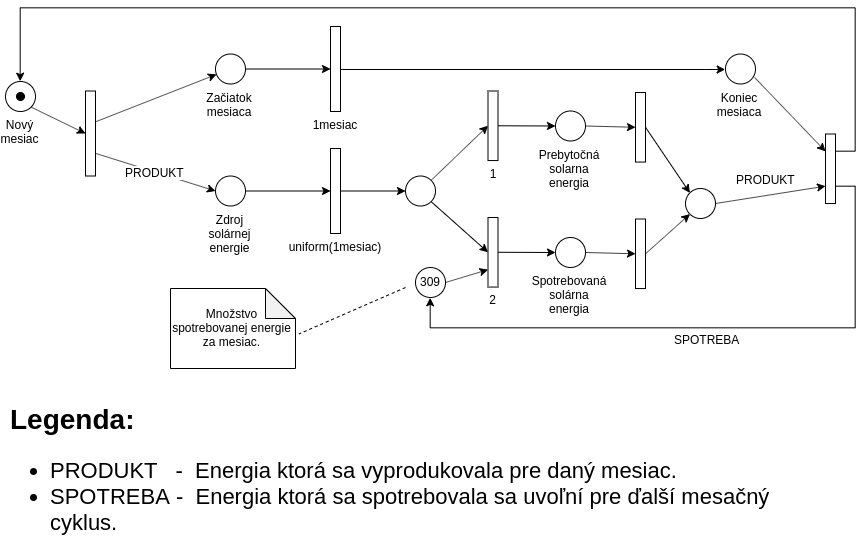
\includegraphics[width=.8\paperwidth]{petri_net.png}
	\caption{Petriho sieť navrhovaného simulačného modelu.}
	\label{obr1}
\end{figure} \label{obr_petri_net}

\newpage
\bibliographystyle{czechiso}
\bibliography{bib}

\end{document}
